\chapter{Impedenzimetro}
\begin{center}
    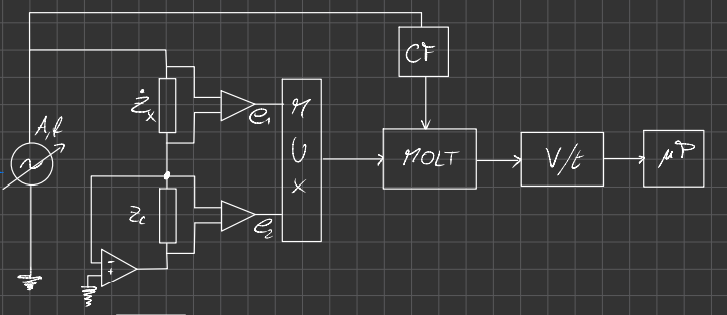
\includegraphics[width=\textwidth]{Images/figure40.png}
\end{center}
Questo strumento serve per misurare \textbf{R, L, C, Q e sfasamenti}, e si basa su una tecnica di tipo \textbf{voltamperometrica}.\\ \\
Esso è composto da:
\begin{itemize}
    \item Un \textbf{generatore di segnale}
    \item \textbf{Impedenza incognita} $Z_x$
    \item \textbf{Resistenza Campione }$Z_x$
    \item \textbf{Amplificatori differenziali} $A_1, A_2$
    \item \textbf{Amplificatore Operazionale} a \textbf{transconduttanza}
\end{itemize}
E vige la seguente equazione:
\begin{equation*}
        Z_x = \frac{E_1}{E_2}R_c
\end{equation*}
In particolare si basa sulla \textbf{tecnica delle proiezioni}:
\begin{center}
    \textbf{Metodo Fast}
\end{center}
\begin{center}
    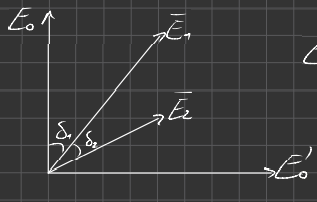
\includegraphics[width=.4\textwidth]{Images/figure41.png}
\end{center}
\begin{equation*}
    E_0 E_1 cos(\delta_1) +    \cancel{ E_0 E_1 cos(2 \w + \delta_1)}\footnote{Perchè il doppia rampa misura solo la parte continua}
\end{equation*}
Misure che fa lo strumento:
\begin{itemize}
    \item $M_1: \; E_0 E_1 cos(\delta_1)$
    \item $M_2: \; E_0 E_2 cos(\delta_2)$
    \item Sfasiamo di 90 gradi $E_0$
    \item $M_3: \; k E_0 E_1 sin(\delta_1)$
    \item $M_4: \; k E_0 E_2 sin(\delta_2)$
\end{itemize}
Sostituendo nell'equazione di $Z_x$ otteniamo:
\begin{equation*}
    \begin{dcases}
        Z_x = \frac{M_1 + j M_3}{M_2 + j M_4} R_c
    \end{dcases}
\end{equation*}
Da questa equazione possiamo ricavarci\textbf{ L, R, C} etc.\\ \\
\begin{center}
    \textbf{Metodo Medium e Slow}
\end{center}
Con questi metodi, molto \textbf{lenti}, otteniamo una \textbf{precisione maggiore}, grazie a misure con \textbf{sfasamenti diversi}.